\subsection{Startup behaviour of the Ozone generator}
\label{sec:ozone}

These are the first experiments conducted using the setup described in
Section~\ref{sec:ozone-setup}. The first goal was to see whether our
setup produced any Ozone at all, i.\,e.\ whether the Silica gel became
permeable for Ozone or not. In a second step we researched the startup
behaviour of our system, as it is important to know the startup time
necessary before our generator reaches a stable Ozone output. Lastly
we checked the influence of the Pen-Ray lamp power on the Ozone
concentration. Using this setup it was impossible to test the
filtering effects on \ch{NO2} produced by the generator. Since the
concentration should be around the \ch{NO_x} concentration in ambient
lab air, it should be no more than a few \si{ppb}. This is far below
the detection limit of a longpath DOAS instrument with a pathlength of
\SI{10}{\centi\meter}. 

Turning on the generator very quickly produced an Ozone signal. Thus
we started a more in depth analysis. Turning of the generator for
about a week and then taking measurements right after turning it on,
we yielded Figure~\ref{fig:long-stop}. As can be seen the generator
takes about \SI{35}{\minute} before it reaches its stable plateau of
around \SI{250}{ppb} Ozone. During this experiment the flow was
constantly set to $\Phi_{\ch{O_3}} = \SI{0.03}{\liter\per\minute}$. It
stands to argue that the startup time could be shortened by increasing
the flow and returning to a lower value later, when the actual \ch{NO_x}
measurements are performed. Furthermore the Hg-lamp power supply was
set\todo{find out current} to \SI{}{A}.

\begin{figure}[htbp]
  \centering
  \begin{tikzpicture}
    \begin{axis}[
      xlabel={Time [\si{\hour}]},
      ylabel={c(\ch{O3}) [ppb]},
      no markers,
      xmin=0,
      xmax=2,
      ]
      \addplot table [col sep=comma] {images/Anschaltkurve2.csv};
    \end{axis}
  \end{tikzpicture}
  \caption{Evolution of Ozone after a long full stop of the
    generator.}
  \label{fig:long-stop}
\end{figure}

Next we were interested in the short term startup behaviour of the
system. We stopped the generator after it had reached a stable level
and restarted it after a fixed time period. The result can be found in
Figure~\ref{fig:multiple-stop}. Since the time resolution of the DOAS
instrument is rather coarse the only safe statement is, that even
after a \SI{4}{\hour} stop the concentration climbed back up to around
\SI{200}{ppb} after \SI{5}{\minute}. So it stands to reason, that if
the device is used regularly the a prolonged startup time should not
be an issue, even if one sticks to the constant flow of
$\Phi_{\ch{O3}} = \SI{0.03}{\liter\per\minute}$. As compared to the
Ozone level in Figure~\ref{fig:long-stop}, the plateau seems to lie
slightly lower in this second experiment. The reason for this lies
most probably in outer conditions such as temperature in the
laboratory, which changed rather drastically from day to day, as the
experiments were conducted in November and December.

\begin{figure}[htbp]
  \centering
  \begin{tikzpicture}
    \begin{axis}[
      xlabel={Time [\si{\minute}]},
      ylabel={c(\ch{O3}) [ppb]},
      legend entries={\nfrac 1/2\si{\hour}, \SI{1}{\hour}, \SI{2}{\hour},
        \SI{4}{\hour}},
      no markers,
      legend pos=south east,
      xmin=0,
      xmax=10,
      ]
      \addplot table [col sep=comma] {images/Multiple-stop.csv};
      \addplot table [col sep=comma,y=1h] {images/Multiple-stop.csv};
      \addplot table [col sep=comma,y=2h] {images/Multiple-stop.csv};
      \addplot table [col sep=comma,y=4h] {images/Multiple-stop.csv};
    \end{axis}
  \end{tikzpicture}
  \caption{Evolution of the Ozone concentration after a full stop of the
    generator.}
  \label{fig:multiple-stop}
\end{figure}

\begin{figure}[htbp]
  \centering
  \begin{tikzpicture}
    \begin{axis}[
      xlabel={Time [\si{\minute}]},
      ylabel={c(\ch{O3}) [ppb]},
      no markers,
      xmin=0,
      xmax=45,
      ]
      \addplot table [col sep=comma] {images/2015-12-02-current2.csv};
    \end{axis}
  \end{tikzpicture}
  \caption{Ozone level dependence on current of Hg-lamp. The steep
    flank occured after a change of the current from to.}
  \label{fig:lamp}
\end{figure}
\todo{enter current in caption}

After having analyzed the startup procedure, we wanted to at least get
the qualitative influence of the power supply current of the Pen-Ray
lamp on the Ozone concentration. Beforehand it was not clear whether a
higher current would increase or decrease the Ozone production rate,
as, as was described in Section~\ref{sec:theory-ozone}, we did not
know how a change in power would transform the power distribution on
the different Mercury lines. We recorded a timeseries while switching
between the two possible currents and yielded
Figure~\ref{fig:lamp}. From this we see that we still work in a regime
where higher power leads to more Ozone. This is interesting to know,
however, since \SI{200}{ppb} is already more than enough Ozone for our
purposes, in the practical application we just used the current
which was easiest to set up\footnote{The currents of all used supplies
  lay in the same region.}.

\subsection{Silica gel influence on \ch{O3} and \ch{NO2} concentration}
\label{sec:silica}

After installing the Ozone generator within a CE-DOAS instrument we
set up an experiment to test its wanted Ozone and its unwanted
\ch{NO2} production. The setup can be found in
Figure~\ref{fig:ozone-flow-setup}. We used to zero air catridges. One
at the zero air input (which also generates the Ozone) and one at the
sample air input. Thus the sample air is \ch{NO2} and \ch{O3}
free. The only way to find these trace gases is, if the Ozone
generater introduced them. Naturally we expect it to produce Ozone
however, we do not want it to produce Nitrogendioxide, which is why we
introduced a Silica filter after the generator. To test the effect of
this filter we took measurements with and without that filter at
different flows of the generator and checked the concentrations.

\begin{figure}[htbp]
  \centering
  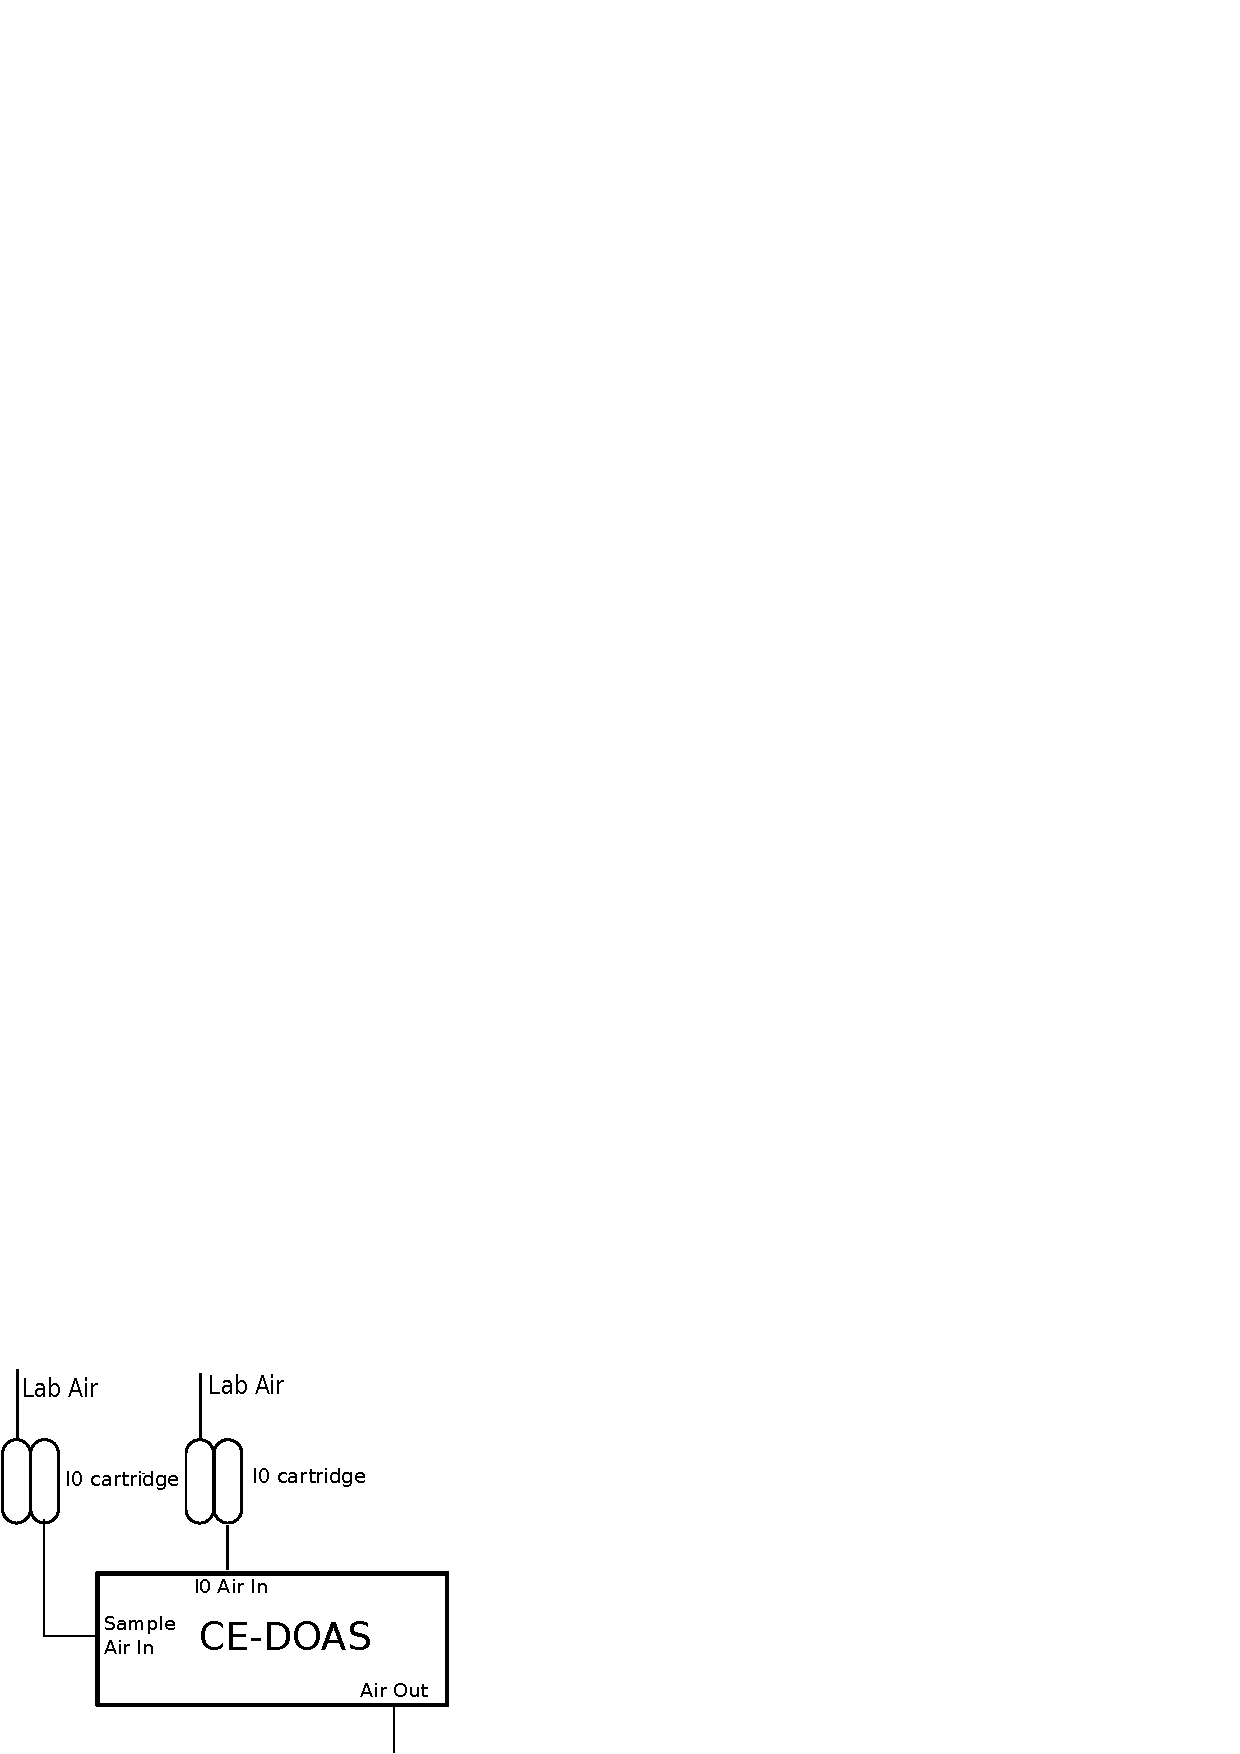
\includegraphics[width=0.35\textwidth]{ozone_setup.png}
  \caption{Ozone measurement setup}
  \label{fig:ozone-flow-setup}
\end{figure}

The result can be found in Figure~\ref{fig:o3-flow}. We see that
changing the flow ascendingly or descendingly does not have an
influence on the \ch{NO2} concentration as long as the silica filter
is in place. In both cases for flows smaller than
\SI{0.2}{\liter\per\minute} the concentration is practically
zero. Only at the very high flow of \SI{0.3}{\liter\per\minute} there
is \ch{NO2} detectable. The difference to the measurement without
Silica filter is obvious. Even the smallest stable flow leads to a
concentration of around \SI{4}{ppb} and for higher flows we soon reach
a stable plateau of about \SI{14}{ppb}. So we see that the Silica
filter is very effective in cleaning the generator air fo \ch{NO2}.

Looking at the Ozone levels we see a rise of the concentration with
the flow as is expected. On strange observation is that both
measurements \emph{with} Silica filter yield higher concentrations
than the measurment \emph{without} Silica filter. This seems
counterintuitive as the Silica gel should also filter some of the
Ozone before it reaches its saturation level. One possible explanation
might be that the silica gel adsorbs \ch{NO2} and other trace gases
fast enough such that they cannot react with the Ozone leading to a
higher Ozone concentration. \todo{Why is the ozone level without filter lower?}

\begin{figure}[htbp]
  \centering
  \includegraphics[width=0.45\textwidth]{O3.png}
  \hfill
  \includegraphics[width=0.45\textwidth]{NO2.png}
  \caption{\ch{O3} and \ch{NO2} concentration over generator flow.}
  \label{fig:o3-flow}
\end{figure}


%%% Local Variables: 
%%% mode: latex
%%% TeX-master: "../Bachelor"
%%% End: 
